\documentclass[11pt,a4paper]{article}
\usepackage[margin=2.3cm]{geometry}
\IfFileExists{lmodern.sty}{\usepackage{lmodern}}{}
\usepackage[T1]{fontenc}
\usepackage{titlesec,tabularx,longtable,booktabs,array,enumitem,xcolor,fancyhdr,amsmath}
\usepackage{listings}
\usepackage{tikz}
\usetikzlibrary{arrows.meta,positioning,fit,calc,shapes.geometric,backgrounds}
\usepackage[hyphens]{url}
\usepackage{hyperref}

\definecolor{headcolor}{RGB}{15,70,60}
\definecolor{boxa}{RGB}{226,239,236}
\definecolor{boxb}{RGB}{238,242,250}
\definecolor{boxc}{RGB}{250,243,230}
\definecolor{boxd}{RGB}{245,245,245}
\definecolor{edge}{RGB}{70,70,70}
\hypersetup{colorlinks=true,linkcolor=headcolor,urlcolor=headcolor,
  pdftitle={TrustBazaar System Design - Unit 6: Chat and Notifications},
  pdfauthor={S. M. Nihal Ahmed, Afrim Hossen Khan, Sabikun Nahar Sinthia}}

\titleformat{\section}{\normalfont\Large\bfseries\color{headcolor}}{\thesection}{10pt}{}
\titleformat{\subsection}{\normalfont\large\bfseries}{\thesubsection}{8pt}{}
\titleformat{\subsubsection}{\normalfont\normalsize\bfseries}{\thesubsubsection}{6pt}{}
\pagestyle{fancy}\fancyhf{}
\fancyhead[L]{System Design Document}\fancyhead[R]{Unit 6: Chat \& Notifications}
\fancyfoot[C]{\thepage}\renewcommand{\headrulewidth}{0.4pt}\setlength{\headheight}{14pt}
\setlength{\emergencystretch}{3em}
\setlength{\parskip}{0.45em}\setlength{\parindent}{0pt}

\lstdefinelanguage{SQLpg}{morekeywords={CREATE,TABLE,TYPE,AS,ENUM,PRIMARY,KEY,REFERENCES,NOT,NULL,DEFAULT,CHECK,UNIQUE,INDEX,ON,WHERE,TRIGGER,BEFORE,INSERT,UPDATE,DELETE,FOR,EACH,ROW,EXECUTE,FUNCTION,RETURNS,LANGUAGE,BEGIN,END,IF,THEN,ELSE,RETURN,SELECT,FROM,INTO,ORDER,BY,DESC,LIMIT,GRANT,REVOKE,TO,SCHEMA,EXTENSION,EXISTS,OR,AND,IN,IS,ALTER,ADD,FOREIGN,GENERATED,ALWAYS,IDENTITY,DEFERRABLE,INITIALLY,DEFERRED,DECLARE,PERFORM,LOOP,RAISE,EXCEPTION,USING,DISTINCT,ROLE,LOGIN,USAGE,ALL,TABLES,STABLE,DO},sensitive=false,morecomment=[l]{--},morestring=[b]'}
\lstdefinelanguage{JS}{morekeywords={import,export,from,const,let,async,await,function,return,new,if,throw,try,catch,for,of,true,false,null},sensitive=true,morecomment=[l]{//},morestring=[b]",morestring=[b]`}
\lstset{basicstyle=\ttfamily\scriptsize,columns=fullflexible,keepspaces=true,breaklines=true,
  keywordstyle=\color{headcolor}\bfseries,commentstyle=\color{gray}\itshape,frame=single,rulecolor=\color{gray!40},
  upquote=true,literate={–}{{--}}1}

\newenvironment{dtable}[1]{\small\begin{longtable}{#1}}{\end{longtable}}

\begin{document}
\begin{titlepage}
\centering
\vspace*{1cm}
{\Large Daffodil International University}\\[0.2cm]
{\large Department of Software Engineering}\\[2cm]
\rule{\linewidth}{0.5pt}\\[0.4cm]
{\huge\bfseries System Design Document}\\[0.3cm]
{\LARGE Unit 6: Chat \& Notifications}\\[0.3cm]
{\large TrustBazaar: A Verified Peer-to-Peer Auction and Marketplace Platform for Used Goods}\\[0.2cm]
\rule{\linewidth}{0.5pt}\\[1.6cm]
{\large S. M. Nihal Ahmed (232-35-002)\\[0.1cm] Afrim Hossen Khan (232-35-076)\\[0.1cm] Sabikun Nahar Sinthia (232-35-475)}\\[1.6cm]
\begin{tabular}{|l|>{\raggedright\arraybackslash}p{8cm}|}
\hline
\textbf{Status} & Draft for team review \\ \hline
\textbf{Version} & 0.1, 18 October 2026 \\ \hline
\textbf{Implements} & SRS v2.0 (\texttt{docs/srs.tex}) \\ \hline
\textbf{Depends on} & Unit 1 (Identity \& Access), Unit 2 (Order, Payment \& Escrow), Unit 3 (Auctions, Listings \& Search); events of Units 1 to 5 \\ \hline
\textbf{Database schema} & \texttt{docs/design/sql/\allowbreak 06\_chat\_notifications.sql}, tested on PostgreSQL (69 checks and concurrency tests, Appendix B) \\ \hline
\end{tabular}
\vfill
\end{titlepage}
\tableofcontents
\newpage
\section{Introduction}

\subsection{Purpose}
This document is the sixth unit of TrustBazaar's System Design Document. It covers the two ways the platform talks to people:
\begin{itemize}[nosep]
  \item \textbf{chat}: one thread per listing and prospective buyer, delivered in real time, with warnings when a message tries to move payment or contact off the platform;
  \item \textbf{notifications}: what every other unit's events mean for the people involved, delivered in the app, by e-mail and, for security notices only, by SMS, including the deadline reminders.
\end{itemize}
Chat matters to trust because one of the defining frauds of the market studied for this project starts there: a fake seller asks for an advance payment and disappears (Supplementary Report, Section~3). The design cannot stop people from typing a phone number, but it can make sure both parties see, on that very message, that payments outside TrustBazaar are not protected (FR-CHT-07).

The unit follows conventions DC-1 to DC-14. It implements ports that earlier units already call: Unit~1's \texttt{NotificationPort} for OTPs and security notices, and a new \texttt{BlockPort} that Units~2 and~3 check before a purchase or a bid.

\subsection{Scope}
\textbf{In scope:}
\begin{itemize}[nosep]
  \item threads, messages, images, delivered and read marks, reconnection;
  \item detection of off-platform payment and contact, and of login details (FR-GAM-20);
  \item blocking, reporting a message, holds for disputes and reports, staff access to threads, retention;
  \item templates in Bangla and English, the channel rules, e-mail and SMS adapters, preferences, the notification history;
  \item auction watching and ending-soon notices, deadline reminders.
\end{itemize}

\textbf{Out of scope, owned by other units:}
\begin{itemize}[nosep]
  \item the live auction channel and the real-time outbid message (Unit~3; this unit keeps the outbid history);
  \item OTP generation, checking and rate limits (Unit~1; this unit only sends the SMS);
  \item the report queue, sanctions and disputes (Unit~7, which places holds on threads through this unit);
  \item the chat and notification screens (Unit~8).
\end{itemize}

\subsection{Requirements covered}
\begin{itemize}[nosep]
  \item \textbf{Functional:} FR-CHT-01 to FR-CHT-10; FR-NTF-01 to FR-NTF-08; FR-GAM-20; FR-TNS-01 and FR-TNS-09 (reports from chat, the reporter's notice); FR-PRV-04 (chat on account closure).
  \item \textbf{Security:} SEC-SES-07 (chat rooms); SEC-ABU-01 (chat limit); SEC-DAT-07 and SEC-DAT-08 (nothing secret in messages sent; image metadata); SEC-INP-04; SEC-LOG-01 (staff reads of chats); SEC-AUTH-09 (OTP delivery).
  \item \textbf{Other:} IF-SW-05, IF-SW-06, IF-COM-02, IF-COM-03; NFR-PERF-04; NFR-SCL-01; DR (chat retention).
\end{itemize}

% ------------------------------------------------------------------
\section{Unit Overview}

\subsection{Responsibilities}
\begin{enumerate}[nosep]
  \item Deliver every chat message exactly once, in order, within a second to an online recipient, and on reconnection to an offline one.
  \item Warn both parties whenever a message looks like a phone number, an account number, a link, an e-mail address, an advance-payment request or login details, without blocking the message.
  \item Let a user block another, and let staff read a thread only for a case that concerns it.
  \item Turn each event of the other units into the right notices, once, on the right channels, in the user's language, and never with anything secret in them.
  \item Remind people of their deadlines in time, and never after the deadline has passed.
\end{enumerate}

\subsection{Components}
\begin{figure}[!htbp]
\centering
\resizebox{\textwidth}{!}{%
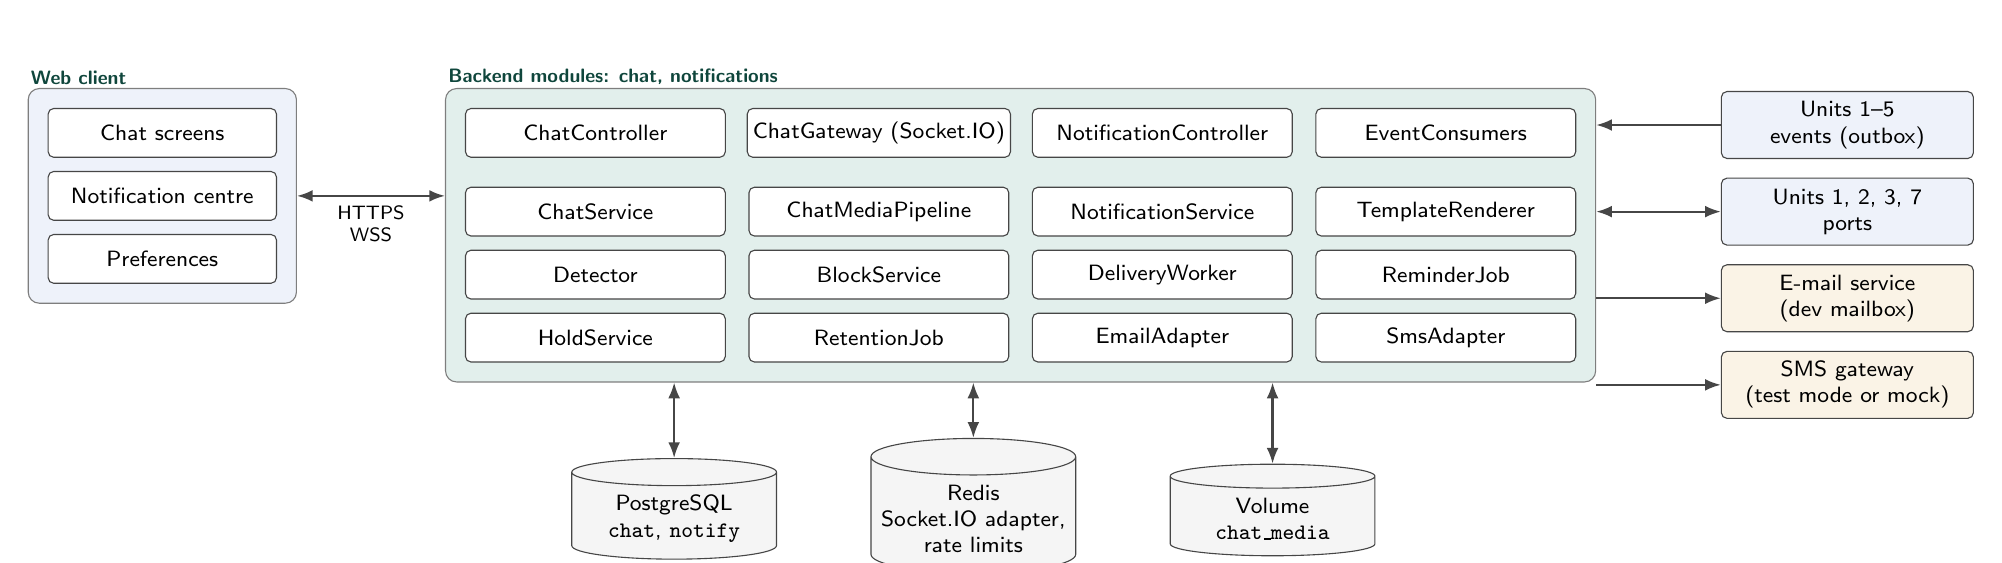
\begin{tikzpicture}[
  font=\sffamily\footnotesize,
  comp/.style={draw=edge, rounded corners=2pt, fill=white, minimum width=3.3cm, minimum height=0.62cm, align=center, inner sep=2pt},
  grp/.style={draw=edge!70, rounded corners=4pt, inner sep=7pt},
  lbl/.style={font=\sffamily\scriptsize\bfseries, text=headcolor, anchor=south west, inner sep=1pt},
  arr/.style={-{Latex[length=2mm]}, draw=edge, thick},
  store/.style={draw=edge, fill=boxd, cylinder, shape border rotate=90, aspect=0.18, minimum width=2.6cm, minimum height=1.1cm, align=center}
]
\node[comp, minimum width=2.9cm] (c1) at (0,3.9) {Chat screens};
\node[comp, minimum width=2.9cm] (c2) at (0,3.1) {Notification centre};
\node[comp, minimum width=2.9cm] (c3) at (0,2.3) {Preferences};
\begin{scope}[on background layer]\node[grp, fill=boxb, fit=(c1)(c3)] (client) {};\end{scope}
\node[lbl] at (client.north west) {Web client};
\foreach \n/\x/\y/\t in {k1/5.5/3.9/ChatController, k2/9.1/3.9/ChatGateway (Socket.IO), k3/12.7/3.9/NotificationController, k4/16.3/3.9/EventConsumers,
  s1/5.5/2.9/ChatService, s2/9.1/2.9/ChatMediaPipeline, s3/12.7/2.9/NotificationService, s4/16.3/2.9/TemplateRenderer,
  s5/5.5/2.1/Detector, s6/9.1/2.1/BlockService, s7/12.7/2.1/DeliveryWorker, s8/16.3/2.1/ReminderJob,
  s9/5.5/1.3/HoldService, s10/9.1/1.3/RetentionJob, s11/12.7/1.3/EmailAdapter, s12/16.3/1.3/SmsAdapter}
  {\node[comp] (\n) at (\x,\y) {\t};}
\begin{scope}[on background layer]\node[grp, fill=boxa, fit=(k1)(k4)(s9)(s12)] (be) {};\end{scope}
\node[lbl] at (be.north west) {Backend modules: chat, notifications};
\node[store] (pg) at (6.5,-1.0) {PostgreSQL\\\texttt{chat}, \texttt{notify}};
\node[store] (rd) at (10.3,-1.0) {Redis\\Socket.IO adapter,\\rate limits};
\node[store] (vol) at (14.1,-1.0) {Volume\\\texttt{chat\_media}};
\node[comp, fill=boxb, minimum height=0.85cm, minimum width=3.2cm] (u1) at (21.4,4.0) {Units 1--5\\events (outbox)};
\node[comp, fill=boxb, minimum height=0.85cm, minimum width=3.2cm] (u7) at (21.4,2.9) {Units 1, 2, 3, 7\\ports};
\node[comp, fill=boxc, minimum height=0.85cm, minimum width=3.2cm] (em) at (21.4,1.8) {E-mail service\\(dev mailbox)};
\node[comp, fill=boxc, minimum height=0.85cm, minimum width=3.2cm] (sm) at (21.4,0.7) {SMS gateway\\(test mode or mock)};
\draw[arr, {Latex[length=2mm]}-{Latex[length=2mm]}] (client.east) -- node[below, font=\sffamily\scriptsize, align=center]{HTTPS\\WSS} (be.west|-client.east);
\foreach \s in {pg, rd, vol}{\draw[arr, {Latex[length=2mm]}-{Latex[length=2mm]}] (\s.north|-be.south) -- (\s.north);}
\draw[arr] (u1.west) -- (be.east|-u1.west);
\draw[arr, {Latex[length=2mm]}-{Latex[length=2mm]}] (be.east|-u7.west) -- (u7.west);
\draw[arr] (be.east|-em.west) -- (em.west);
\draw[arr] (be.east|-sm.west) -- (sm.west);
\end{tikzpicture}}
\caption{Components of the Chat \& Notifications unit. Messages between backend instances pass through the Socket.IO Redis adapter; e-mail and SMS leave only through the two adapters.}
\label{fig:components}
\end{figure}

\begin{dtable}{@{}>{\raggedright\arraybackslash}p{3.8cm}>{\raggedright\arraybackslash}p{11.4cm}@{}}
\toprule
\textbf{Component} & \textbf{Responsibility} \\ \midrule \endhead
ChatService & Opens threads, posts messages through \texttt{chat.post}, applies the chat rate limit (CP-35), syncs history (Section~\ref{sec:chat}). \\
ChatGateway & Socket.IO events for chat and notifications on the authenticated connection; rooms \texttt{user:\{id\}} only (SEC-SES-07). \\
ChatMediaPipeline & Checks, strips and re-encodes chat images, stores them privately, issues signed links to participants (Section~\ref{sec:images}). \\
Detector & The rules of Section~\ref{sec:detect}; the database function \texttt{chat.detect} is the implementation used on every message. \\
BlockService & Blocks and unblocks; implements \texttt{BlockPort} for Units~2 and~3 (Section~\ref{sec:block}). \\
HoldService, RetentionJob & Holds for disputes and reports; staff reads; the retention purge (Section~\ref{sec:holds}). \\
EventConsumers & One idempotent consumer per event type of Units~1 to~5; each maps an event to notices and reminders (Section~\ref{sec:map}). \\
NotificationService, TemplateRenderer & Creates notifications through \texttt{notify.create}; renders the template in the recipient's language at read or send time. \\
DeliveryWorker, adapters & Sends pending e-mail and SMS with retries; the adapters are the only code that talks to the providers (Section~\ref{sec:channels}). \\
ReminderJob & Claims due reminders, checks with the owning unit that the deadline still applies, and sends them (Section~\ref{sec:reminders}). \\
\bottomrule
\end{dtable}
\section{Interfaces}

\subsection{HTTP API}
\label{sec:api}
All paths are under \texttt{/api/v1}; policies and rate limits are those of Unit~1. Another user is shown only by display name and badge (FR-ACC-10).

{\small
\begin{longtable}{@{}>{\ttfamily\raggedright\arraybackslash}p{1.55cm}>{\ttfamily\raggedright\arraybackslash}p{4.8cm}>{\raggedright\arraybackslash}p{2.4cm}>{\raggedright\arraybackslash}p{6.1cm}@{}}
\toprule
\textnormal{\textbf{Method}} & \textnormal{\textbf{Path}} & \textbf{Policy} & \textbf{Purpose (requirement)} \\ \midrule \endhead
\multicolumn{4}{@{}l}{\textbf{Chat}} \\
POST & /\allowbreak listings/\allowbreak \{id\}/\allowbreak threads & SignedIn & Open (or find) my thread with the seller (FR-CHT-01) \\
GET & /\allowbreak threads & SignedIn & My threads, newest first, with unread counts \\
GET & /\allowbreak threads/\allowbreak \{id\}/\allowbreak messages?\allowbreak after= & Participant & Messages after a sequence number; used to resync (FR-CHT-02, IF-COM-02) \\
POST & /\allowbreak threads/\allowbreak \{id\}/\allowbreak messages & Participant & Send text, with the client's message id (FR-CHT-02) \\
POST & /\allowbreak threads/\allowbreak \{id\}/\allowbreak images & Participant & Send an image (FR-CHT-03) \\
POST & /\allowbreak threads/\allowbreak \{id\}/\allowbreak marks & Participant & Delivered and read up to (FR-CHT-05) \\
POST & /\allowbreak threads/\allowbreak \{id\}/\allowbreak reports & Participant & Report the thread or a message (FR-CHT-06) \\
POST, DELETE & /\allowbreak blocks/\allowbreak \{userId\} & SignedIn & Block or unblock a user (FR-CHT-08) \\
\multicolumn{4}{@{}l}{\textbf{Notifications}} \\
GET & /\allowbreak notifications & SignedIn & History, newest first; cursor (FR-NTF-04) \\
POST & /\allowbreak notifications/\allowbreak read & SignedIn & Mark some or all as read \\
GET, PUT & /\allowbreak me/\allowbreak notification-\allowbreak preferences & SignedIn & Language; transactional e-mails on or off (FR-NTF-05) \\
POST, DELETE & /\allowbreak listings/\allowbreak \{id\}/\allowbreak watch & SignedIn & Watch an auction (FR-NTF-02) \\
\multicolumn{4}{@{}l}{\textbf{Providers and staff}} \\
POST & /\allowbreak webhooks/\allowbreak sms/\allowbreak \{provider\}, /\allowbreak webhooks/\allowbreak email/\allowbreak \{provider\} & Provider signature & Delivery receipts and bounces (IF-COM-03) \\
GET & /\allowbreak staff/\allowbreak cases/\allowbreak \{type\}/\allowbreak \{caseId\}/\allowbreak threads/\allowbreak \{id\} & Staff(operator), case & Read a thread for a case that holds it; logged (FR-CHT-10) \\
POST, DELETE & /\allowbreak staff/\allowbreak chat/\allowbreak detection-\allowbreak terms & Staff(operator) & Maintain the detection terms \\
POST, PATCH & /\allowbreak admin/\allowbreak notification-\allowbreak templates & Staff(admin) & New template versions \\
\bottomrule
\end{longtable}
}

\subsection{Live channel}
The Socket.IO connection authenticated by Unit~1 (SEC-SES-07) joins only the room \texttt{user:\{id\}} for chat and notifications; there are no thread rooms, so a user can never be subscribed to a thread they are not in.
\begin{dtable}{@{}>{\ttfamily}p{3.9cm}>{\raggedright\arraybackslash}p{11.3cm}@{}}
\toprule
\textnormal{\textbf{Message}} & \textbf{Content and use} \\ \midrule \endhead
chat.message & To both participants after commit: thread, sequence number, sender, kind, text or a signed image link, flags. The client applies messages in sequence order and, on a gap, fetches the missing ones. \\
chat.ack (client to server) & ``Delivered up to'' as soon as a message arrives, ``read up to'' when it is shown. \\
chat.marks & To the sender: the other side's new delivered and read marks. \\
notification.new & The new notification's id, title in the user's language and the unread count. \\
\bottomrule
\end{dtable}

\subsection{Ports provided}
\begin{lstlisting}[language=Java,morekeywords={interface,type,Promise,string,boolean,number,bigint}]
interface NotificationPort {                       // used by Unit 1 (Unit 1 Section 2)
  sendSms(phone: string, purpose: 'otp' | 'security_notice', template: string, vars: object): Promise<void>;
  sendEmail(address: string, template: string, vars: object): Promise<void>;   // links (verification, reset)
}
interface BlockPort {                              // used by Units 2 and 3 (FR-CHT-08)
  assertNotBlocked(sellerId: string, buyerId: string): Promise<void>;          // throws 'blocked'
}
interface ChatCommands {                           // used by Unit 7
  hold(threadId: string, caseType: 'dispute' | 'report', caseId: string): Promise<void>;
  release(threadId: string, caseType: 'dispute' | 'report', caseId: string): Promise<void>;
  threadFor(listingId: string, buyerId: string): Promise<string | null>;      // the thread of an order
}
interface Notifier {                               // used by Unit 7 (decisions, FR-TNS-09)
  notify(userId: string, template: string, params: object, dedupeKey: string): Promise<void>;
}
\end{lstlisting}

\subsection{Events consumed}
\label{sec:map}
Each event of another unit maps to notices for the people concerned. Every consumer is idempotent: the dedupe key is the event's id, the recipient and the template, so an event delivered twice creates one notice (DC-6).
\begin{dtable}{@{}>{\raggedright\arraybackslash}p{5.9cm}>{\raggedright\arraybackslash}p{4.6cm}>{\raggedright\arraybackslash}p{4.7cm}@{}}
\toprule
\textbf{Events} & \textbf{Notice to, channels} & \textbf{Reminders scheduled or cancelled} \\ \midrule \endhead
\texttt{identity.signin.new\_device}, \texttt{.password.changed}, \texttt{.contact.changed}, \texttt{.mfa.*}; \texttt{payments.payout\_account.changed} & The user; app, e-mail, SMS; cannot be switched off (FR-NTF-06) & --- \\
\texttt{identity.kyc.verified}, \texttt{.rejected}, \texttt{.account.suspended}, \texttt{.reinstated} & The user; app, e-mail (FR-NTF-03, FR-TNS-03) & --- \\
\texttt{orders.order.created} (auction or second chance) & Buyer & payment window \\
\texttt{orders.order.paid} & Buyer and seller; app, e-mail & cancel payment window; schedule meetup, pickup or credential deadline \\
\texttt{orders.order.delivered} & Buyer and seller & dispute window (physical) \\
\texttt{orders.escrow.released}, \texttt{.refunded}, \texttt{.partially\_refunded}, \texttt{.frozen} & Buyer and seller & cancel all for the order \\
\texttt{payments.payout.*}, \texttt{payments.refund.*} & The payee & --- \\
\texttt{listings.listing.published}, \texttt{.removed}; \texttt{game\_accounts.ownership.*} & Seller (FR-NTF-03) & --- \\
\texttt{auctions.bid.outbid} & Previous leader; app history only (live message is Unit~3's) & --- \\
\texttt{auctions.auction.awarded}, \texttt{.unsold}, \texttt{.offer.*} & Winner, seller, bidders & payment window (second chance) \\
\texttt{delivery.meetup.*}, \texttt{.handover.*}, \texttt{.shipment.status\_changed} & The other party, or both (FR-NTF-03) & cancel meetup or pickup on completion \\
\texttt{game\_accounts.credentials.*}, \texttt{.rekey.*}, \texttt{.takeover.completed} & Seller or buyer & credential deadline; takeover window (re-armed by a re-key); protection period \\
Unit~7 dispute and report events & Both parties; the reporter (FR-TNS-09) & --- \\
\bottomrule
\end{dtable}
Ending-soon notices (FR-NTF-02) are not event-driven: the reminder job asks Unit~3 for auctions ending within CP-38 (5~minutes) and notifies their watchers and bidders once.

\subsection{Ports required}
\begin{dtable}{@{}>{\raggedright\arraybackslash}p{4.6cm}>{\raggedright\arraybackslash}p{10.6cm}@{}}
\toprule
\textbf{Port} & \textbf{Provider and use} \\ \midrule \endhead
\texttt{IdentityQuery} (Unit 1) & Display names and badges; new \texttt{getContact(userId)} for the e-mail address and number at send time, so contact details are never stored with a notification (I-36). \\
\texttt{FileVault} (Unit 1) & Image re-encoding and metadata removal, reused for chat images on their own volume. \\
\texttt{ListingsQueries}, \texttt{AuctionQuery} (Unit 3) & The listing and seller of a new thread; auctions ending soon and their bidders (I-38). \\
Deadline queries (Units 2, 4, 5) & Before sending a reminder: does the deadline still apply? (Section~\ref{sec:reminders}). \\
\texttt{ReportCommands} (Unit 7) & File a report from chat into the report queue (FR-CHT-06, FR-TNS-01). \\
\texttt{RateLimiter}, \texttt{AuditService}, \texttt{ConfigPort}, \texttt{Clock} & Chat limit CP-35; audit of staff reads; parameters; time. \\
\bottomrule
\end{dtable}
\section{Data Design}
\label{sec:data}
The schema is in \texttt{docs/design/sql/06\_chat\_notifications.sql} (Appendix~\ref{app:ddl}), loaded after Units~1 to~5. The unit owns two schemas, \texttt{chat} and \texttt{notify}. Its foreign keys point to users and staff (Unit~1) and listings (Unit~3). Orders and cases of later units are referenced by plain ids (DC-5).

\tikzset{
  ent/.style={draw=edge, fill=white, rounded corners=1.5pt, align=left, inner sep=3pt, font=\sffamily\scriptsize, text width=3.9cm},
  fk/.style={-{Latex[length=1.6mm]}, draw=edge!80, semithick},
}
\newcommand{\ent}[2]{\textbf{\color{headcolor}#1}\\[-1pt]{\ttfamily\tiny #2}}
\begin{figure}[!htbp]
\centering
\resizebox{0.98\textwidth}{!}{%
\begin{tikzpicture}
\node[ent, fill=boxd] (lst) at (0,6.4) {\ent{listings.listings}{(Unit 3)}};
\node[ent, fill=boxa, text width=4.4cm] (th) at (0,3.6) {\ent{chat.threads}{listing, buyer, seller (unique pair)\\last\_seq, last\_message\_at\\delivered / read marks per side\\purged\_at}};
\node[ent, fill=boxa] (m) at (5.4,3.6) {\ent{chat.messages}{(thread, seq) unique\\sender, client\_msg\_id\\kind, body or image\_key\\flags (detection)}};
\node[ent] (bl) at (5.4,6.4) {\ent{chat.blocks}{blocker, blocked}};
\node[ent] (ho) at (0,0.9) {\ent{chat.thread\_holds}{thread, case type, case id\\released\_at}};
\node[ent] (sa) at (5.4,0.9) {\ent{chat.staff\_access\_log}{staff, thread, case, at\\(append-only)}};
\node[ent] (dt) at (10.6,6.4) {\ent{chat.detection\_terms}{term (NFC, lower), flag}};
\node[ent, fill=boxb] (tp) at (10.6,3.9) {\ent{notify.templates}{(code, version), category\\channels, allowed\_params\\titles and bodies, bn and en}};
\node[ent, fill=boxb] (n) at (15.8,3.9) {\ent{notify.notifications}{user, template, params\\dedupe\_key (unique per user)\\read\_at}};
\node[ent] (dv) at (15.8,1.4) {\ent{notify.deliveries}{(notification, channel)\\status, attempts, provider\_ref}};
\node[ent] (rm) at (10.6,1.4) {\ent{notify.reminders}{user, kind, subject, lead\\due\_at, fire\_at, status}};
\node[ent] (ot) at (15.8,6.4) {\ent{notify.preferences, watches,}{sms\_log, chat\_email\_state}};
\draw[fk] (th.north) -- (lst.south);
\draw[fk] (m.west) -- (th.east|-m.west);
\draw[fk] (ho.north) -- (th.south);
\draw[fk] (sa.west) -- ++(-0.5,0) |- ([yshift=-12pt]th.east);
\draw[fk] (n.west) -- (tp.east|-n.west);
\draw[fk] (dv.north) -- (n.south);
\end{tikzpicture}}
\caption{The \texttt{chat} and \texttt{notify} schemas. User references are omitted.}
\label{fig:er}
\end{figure}

\subsection{Tables and rules the database enforces}
\begin{dtable}{@{}>{\ttfamily\raggedright\arraybackslash}p{3.7cm}>{\raggedright\arraybackslash}p{11.5cm}@{}}
\toprule
\textnormal{\textbf{Table}} & \textbf{Rules enforced by the database} \\ \midrule \endhead
chat.threads & One per listing and buyer; buyer is not the seller; parties fixed. Sequence and delivered and read marks only move forward; read $\le$ delivered $\le$ last message. Nothing can be added once purged. \\
chat.messages & Unique sequence number per thread, and unique client id per sender, so a resend is recognised. Text is plain, without control characters, and not empty; an image needs a stored image. Messages can never be edited or deleted; at the end of retention only their content is removed. \\
chat.blocks & Not oneself; while a block exists in either direction, no message and no new thread between the two. \\
chat.thread\_holds, chat.\allowbreak staff\_access\_log & Staff read a thread only through a live hold of the same case; each read is logged; the log is append-only. \\
chat.detection\_terms & Stored lower case and NFC-normalised. \\
notify.templates & SMS only for security notices; security notices always by SMS and e-mail; one active version per code. \\
notify.notifications & One per user and dedupe key. Parameters only those the template declares, as plain values, and none that contains a phone number, e-mail address, NID-like number or six-digit code (trigger). \\
notify.deliveries & One per notification and channel; a sent delivery records when. \\
notify.reminders & One per user, kind, subject and lead time; fire time $=$ deadline $-$ lead. \\
\bottomrule
\end{dtable}

% ------------------------------------------------------------------
\section{Chat}
\label{sec:chat}

\subsection{Threads}
A thread belongs to one listing and one prospective buyer, with the listing's seller (FR-CHT-01). It is opened only from a listing page, by a signed-in user who is not the seller; \texttt{chat.open\_thread} returns the existing thread if there is one, so ten simultaneous requests produced one thread. The same thread continues after a purchase, so the conversation before and after the sale is in one place for both parties and, if needed, for a dispute.

\subsection{Sending and delivery}
\begin{enumerate}[nosep]
  \item The client gives every message a random id before sending. If the network fails and the client sends again, the database recognises the id and returns the original message (tested: ten simultaneous resends stored one message).
  \item \texttt{chat.post} locks the thread, checks that the sender is a participant and that no block exists, gives the message the next sequence number, runs the detector, and stores the message with its flags. Inside the database this takes about 0.33~ms (1{,}000 messages; three runs 0.32--0.36~ms), and twenty simultaneous posts got sequence numbers 1 to 20 with no gap or repeat.
  \item After commit, the gateway emits \texttt{chat.message} to \texttt{user:\{buyer\}} and \texttt{user:\{seller\}} through the Redis adapter, so it reaches the recipient on whichever backend instance holds the connection (NFR-PERF-04, NFR-SCL-01).
  \item The recipient's client acknowledges ``delivered up to $n$'' on arrival and ``read up to $n$'' when shown. The marks only move forward, so acknowledgements arriving out of order cannot move them back (tested with twenty simultaneous acknowledgements).
\end{enumerate}
Sequence numbers make reconnection simple (FR-CHT-02, IF-COM-02). A client that was offline asks for each thread's messages after the last sequence number it holds, in pages of DV-44 (200). A client that sees a gap in the live stream fetches the missing range. Delivered and read indicators (FR-CHT-05) are derived from the marks: a message is delivered if its number is at or below the recipient's delivered mark.

Chat is limited to 30 messages per minute per user (CP-35, SEC-ABU-01) by Unit~1's shared rate limiter.

\subsection{Text and images}
\label{sec:images}
Messages are plain text of at most 2{,}000 characters (DV-40). The client renders them as text only, never as HTML, and web addresses are shown as non-clickable text with a warning (FR-CHT-09). Images go through the same checks as KYC images in Unit~1's \texttt{FileVault}: type identified from content, size limit CP-33, decoded, rotated upright, all metadata including location removed, re-encoded (FR-CHT-03, SEC-INP-04, SEC-DAT-08). They are stored on a private \texttt{chat\_media} volume and shown only to the two participants through signed links valid for CP-31.

\subsection{Detecting off-platform payment and contact}
\label{sec:detect}
Every message passes through \texttt{chat.detect}, which returns flags. A flagged message is still delivered (FR-CHT-07), but both participants see a warning on it: \emph{``Payments made outside TrustBazaar are not protected. Pay only through the app.''} The flags and their tests are:
\begin{dtable}{@{}>{\ttfamily\raggedright\arraybackslash}p{3.2cm}>{\raggedright\arraybackslash}p{7.6cm}>{\raggedright\arraybackslash}p{4.4cm}@{}}
\toprule
\textnormal{\textbf{Flag}} & \textbf{Detected as} & \textbf{Tested with} \\ \midrule \endhead
phone & An 11-digit Bangladeshi mobile number (\texttt{01[3-9]}\ldots), with or without 88 or 880, also written in Bangla digits or split by spaces, dots or dashes. bKash, Nagad and Rocket wallets are mobile numbers. & \texttt{01711-234567} in Bangla digits; \texttt{+880 1811 234 567} \\
account\_number & Any other run of 10 to 20 digits, after joining separated groups. & \texttt{A/C 1234 5678 9012 34}; not a price or a year \\
link & A web address or a short-link or messaging domain (\texttt{wa.me}, \texttt{t.me}). & \texttt{www.my-shop.com} \\
email & An e-mail address. & \texttt{a.b@example.com} \\
payment\_phrase & A detection term asking for advance or direct payment, in Bangla or English. & \emph{agrim}, \emph{age taka}, ``pay first'' \\
off\_platform\_app & A term naming another messaging app. & WhatsApp, imo, Telegram \\
credentials & A term for login details (FR-GAM-20): the seller is directed to the sealed handover of Unit~5. & ``login id'', ``pass:'', \emph{password} in Bangla \\
\bottomrule
\end{dtable}
Before matching, the text is NFC-normalised, lower-cased, and Bangla digits are read as digits. English terms must stand as whole words, so ``kimono'' does not match ``imo'' and ``advanced'' does not match ``advance'' (tested). Bangla terms match as substrings, because the regular-expression engine does not treat Bangla vowel signs as word characters.

The terms are data, maintained by operators, and seeded with 31 Bangla and English terms (DV-45). False positives are accepted by design: a buyer who writes ``I will pay with bKash in the app'' sees the warning too. Because a flag only adds a warning and never blocks, a false positive costs a sentence of reading, while a missed scam costs money. Flagged messages also raise \texttt{chat.message.flagged}, which Unit~7 can use as a Trust \& Safety signal; the event carries the flags, not the text.

\subsection{Blocking}
\label{sec:block}
A user can block another (FR-CHT-08). While a block exists in either direction:
\begin{itemize}[nosep]
  \item no message can be sent in either direction, and no new thread opened between them (database rule; the blocker unblocks to talk again);
  \item the blocked user cannot bid on the blocker's auctions or buy from the blocker. Units~2 and~3 call \texttt{BlockPort.assertNotBlocked} before checkout and before a bid (I-37, I-38).
\end{itemize}
Orders already paid continue (FR-CHT-08). They need no chat: the meetup proposals and handover code (Unit~4), the sealed handover (Unit~5) and disputes (Unit~7) all work in the order view.

The bid check is made by the service before it calls \texttt{auctions.place\_bid}, not inside that function, because the bid engine must not read another unit's tables (DC-1). A bid placed in the same instant as the block can therefore still be accepted. This is acceptable: a block protects against unwanted contact, not against a money invariant.

\subsection{Reports, holds and staff access}
\label{sec:holds}
A participant can report a thread or a message (FR-CHT-06). The report goes to Unit~7's queue through \texttt{ReportCommands}, and Unit~7 places a \emph{hold} on the thread for that case. A dispute on an order places a hold on its thread in the same way. A hold has two effects:
\begin{itemize}[nosep]
  \item the thread is kept beyond the retention period while the case is open (FR-CHT-04);
  \item it is the only ground on which an operator may read the thread. \texttt{chat.staff\_read} requires a live hold of the very case the operator is working on, and logs every read (FR-CHT-10, SEC-LOG-01). An operator with a different case, or after the hold is released, is refused (tested).
\end{itemize}

\subsection{Retention and closed accounts}
A thread is kept for 1 year after its last message (SRS retention schedule). The retention job then removes the content of every message (text and image) and returns the image keys so the files can be deleted, unless a hold is live. The thread row and message metadata stay, so sequence numbers and the staff access log still make sense. When an account closes, the other party sees the closed user's name as ``Closed account''. The content stays until the thread's retention ends, because it is also the other party's record (FR-PRV-04 permits data kept under the retention schedule).
\section{Notifications}
\label{sec:notify}

\subsection{From event to notice}
\begin{enumerate}[nosep]
  \item An event arrives from another unit's outbox (at least once, DC-6).
  \item Its consumer decides the recipients and the template (Section~\ref{sec:map}), and calls \texttt{notify.create} with a dedupe key made of the event id, the recipient and the template. A second delivery of the same event creates nothing; ten simultaneous deliveries created one notification and one e-mail delivery (tested).
  \item \texttt{notify.create} stores the notification for the in-app history and adds one delivery row per further channel, according to the template and the user's preferences.
  \item After commit, the gateway pushes \texttt{notification.new} to the user's room. The delivery worker sends the e-mail and SMS rows.
\end{enumerate}
Notifications store the template and its parameters, not rendered text. The text is rendered in the recipient's language, Bangla by default, when shown or sent. A corrected template version therefore applies to the history too, and nothing personal is stored twice.

\subsection{Channels}
\label{sec:channels}
\begin{dtable}{@{}>{\raggedright\arraybackslash}p{3.4cm}>{\raggedright\arraybackslash}p{2.3cm}>{\raggedright\arraybackslash}p{2.3cm}>{\raggedright\arraybackslash}p{7.0cm}@{}}
\toprule
\textbf{Category} & \textbf{In app} & \textbf{E-mail} & \textbf{SMS} \\ \midrule \endhead
Security (FR-NTF-06) & always & always & always; cannot be switched off \\
Transaction, account (FR-NTF-03) & always & unless turned off & never \\
Chat & always & coalesced (DV-41) & never \\
Auction, reminder & always & unless turned off & never \\
OTP (Unit~1) & --- & --- & sent synchronously; no notification row; content never stored \\
\bottomrule
\end{dtable}
The database enforces the SMS rule (FR-NTF-05): a template that is not a security notice cannot list SMS, and a security template must list both SMS and e-mail. A user who turns transactional e-mails off still gets security e-mails and SMS (tested).

\begin{itemize}[nosep]
  \item \textbf{E-mail} (IF-SW-06) goes through an adapter for SMTP or a provider API. In the academic deliverable, and in every sandbox build, the adapter writes each message to a development mailbox inside the backend, viewable on a staff-only page and labelled as simulated. This keeps within the four containers of NFR-MNT-01. E-mails are plain text with a simple HTML part, contain links only to TrustBazaar's own domain, and carry no tracking pixel. Production needs SPF, DKIM and DMARC on the sending domain.
  \item \textbf{SMS} (IF-SW-05) goes through an adapter for a gateway with a test mode, or a logged mock labelled as simulated (AS-4). The SMS log records an HMAC of the number, the purpose (OTP or security notice), the status and the provider reference, never the text. This keeps OTPs out of the database entirely (SEC-AUTH-09, SEC-DAT-07).
  \item \textbf{Retries.} Failed deliveries are retried with exponential backoff and jitter, from 1~minute to 30~minutes, six attempts (DV-43). A security notice that finally fails is shown to an operator. Provider receipts and bounces arrive on signed webhook endpoints (IF-COM-03).
  \item \textbf{Addresses at send time.} The e-mail address and number are fetched from Unit~1 when the delivery is sent, so a change of contact takes effect at once. A contact-change notice goes to the old contact, as Unit~1 requires.
\end{itemize}

\subsection{Nothing secret in a notice}
FR-NTF-08 forbids passwords, OTPs, game-account credentials, full NID numbers and other users' contact details in any notification. The design has three layers:
\begin{enumerate}[nosep]
  \item \textbf{Declared parameters.} Each template lists the parameters it may carry, and the database refuses any other, and any nested value (tested). No template declares a parameter for a password, credential, NID or contact.
  \item \textbf{A content check.} The database also refuses a parameter that contains a phone number (including Bangla digits and separators), an e-mail address, a 10-, 13- or 17-digit number (the NID formats) or a six-digit code (tested). Amounts are passed as numbers, so they are not affected.
  \item \textbf{Masking user text.} Listing titles and display names are written by users and may contain a phone number. The consumers pass them through \texttt{notify.mask}, which replaces such content with ``[hidden]''.
\end{enumerate}
Chat notices never quote the message: they say ``New message from Rahim about Used phone'', because the message itself may hold a phone number and a lock-screen preview is visible to anyone nearby.

\subsection{Chat e-mails}
A new chat message always produces an in-app notice. It produces an e-mail only if the recipient is not connected at that moment and has had no chat e-mail for that thread in the last 15~minutes (DV-41). This keeps a lively conversation from producing dozens of e-mails.

\subsection{Auctions}
The live outbid message is Unit~3's (FR-NTF-01). This unit adds it to the history. For FR-NTF-02, users can watch an auction. Every minute, the reminder job asks Unit~3 for auctions ending within CP-38 (5~minutes) and notifies their watchers and bidders, once per auction and user (dedupe key).

\subsection{Deadline reminders}
\label{sec:reminders}
FR-NTF-07 asks for reminders 24~hours and 2~hours before each deadline (CP-38): the payment window, meetup handover, courier pickup, credential delivery, takeover window, dispute window and protection period.
\begin{itemize}[nosep]
  \item \textbf{Scheduling.} The consumers schedule two reminders per deadline from the event that sets it. A deadline that moves reschedules its reminders instead of adding new ones. A deadline that moves later re-arms a reminder already sent, for example when a re-key restarts the takeover window (tested).
  \item \textbf{Cancelling.} The event that completes the step cancels the remaining reminders for it, for example \texttt{orders.order.paid} for the payment window.
  \item \textbf{Sending.} The job claims due reminders with \texttt{FOR UPDATE SKIP LOCKED}. Five job instances claiming 50 due reminders at the same moment sent each exactly once (tested). A reminder whose deadline has already passed is cancelled, never sent. Before sending, the job asks the owning unit whether the deadline still applies, so a reminder that missed its cancellation event is dropped rather than sent.
\end{itemize}
\section{Scheduled Jobs}
\label{sec:jobs}
\begin{dtable}{@{}>{\raggedright\arraybackslash}p{3.6cm}>{\raggedright\arraybackslash}p{1.8cm}>{\raggedright\arraybackslash}p{9.8cm}@{}}
\toprule
\textbf{Job} & \textbf{Every} & \textbf{Action} \\ \midrule \endhead
Delivery worker & continuous & Send pending e-mail and SMS deliveries; retry failed ones (DV-43). \\
Reminders and ending-soon & 1 min & Claim due reminders, verify, send; ending-soon notices (FR-NTF-02, FR-NTF-07). \\
Chat retention & daily & \texttt{chat.purge\_due(1 year)}; delete the returned image files. \\
Notification retention & daily & Delete in-app history older than 1 year, and delivery and SMS records older than 90 days (DV-42). \\
\bottomrule
\end{dtable}

\section{Performance and Scaling}
\begin{itemize}[nosep]
  \item \textbf{Chat latency} (NFR-PERF-04, 1~s p95). The path is: authenticated socket, rate-limit counter in Redis, one database call (about 0.33~ms inside the database), commit, and one emit through the Redis adapter to the two user rooms. No step waits on e-mail or SMS, which are sent afterwards by the worker.
  \item \textbf{Several instances} (NFR-SCL-01). No instance holds chat state: sequence numbers come from the database, rooms are joined per connection, and messages between instances pass through Redis. Jobs use \texttt{SKIP LOCKED}.
  \item \textbf{Restart.} Messages are committed before they are emitted, so a restart loses only connections; clients reconnect and fetch after their last sequence number (IF-COM-02).
  \item \textbf{Load test} (to run with the built application): 500 signed-in users with chat open, 50 messages per second across 100 threads, measuring sender-to-recipient time at the clients; and a burst of 5{,}000 notifications from one event storm, measuring the time to the last in-app push.
\end{itemize}

\section{Security and Privacy}
\begin{itemize}[nosep]
  \item \textbf{Who can read a thread.} Only its two participants: the database checks the sender of every message and every acknowledgement, and the socket joins only the user's own room (SEC-SES-07). Staff read only through a held case, and every read is logged (FR-CHT-10).
  \item \textbf{Content safety.} Plain text only, rendered as text; links shown inert; images re-encoded without metadata and served through signed links to participants only (SEC-INP-04, SEC-DAT-08).
  \item \textbf{Fraud signals.} Off-platform and credential warnings on the message itself, for both parties; flags, not text, go to Trust \& Safety.
  \item \textbf{Notices.} No secret in a notice (three layers), no message text in chat notices, no OTP or SMS text stored, contact details fetched at send time.
  \item \textbf{Abuse limits.} Chat 30 messages per minute (CP-35); reports 20 per day (CP-35); OTP send limits stay in Unit~1 (CP-05). Retries and coalescing keep a fault from flooding a user's inbox.
  \item \textbf{Integrity.} Messages cannot be edited or deleted by anyone; only retention removes their content. The staff access log is append-only, and the application role cannot change it or delete messages (tested).
\end{itemize}

\section{Parameters}
\textbf{SRS parameters used:} CP-05 (OTP sends, applied by Unit~1); CP-31 (signed links); CP-33 (image size); CP-35 (chat and report limits); CP-38 (lead times); CP-41 (closure).

\textbf{Design values introduced} (continuing DV-1 to DV-39):
\begin{dtable}{@{}>{\bfseries}p{1.3cm}>{\raggedright\arraybackslash}p{4.6cm}>{\raggedright\arraybackslash}p{4.6cm}>{\raggedright\arraybackslash}p{4.4cm}@{}}
\toprule
\textnormal{\textbf{ID}} & \textbf{Value} & \textbf{Default} & \textbf{Reason} \\ \midrule \endhead
DV-40 & Message size & 2{,}000 characters; image caption 300; one image per message & Chat, not documents. \\
DV-41 & Chat e-mail coalescing & at most one per thread per 15 min, only when offline & No inbox flooding. \\
DV-42 & Notification retention & in-app history 1 year; delivery and SMS records 90 days & Not in the SRS schedule (I-42). \\
DV-43 & E-mail and SMS retries & 1 min doubling to 30 min; 6 attempts & Then failed; security failures to an operator. \\
DV-44 & Sync page size & 200 messages; 50 notifications & Fast reconnect on mobile. \\
DV-45 & Detection terms & 31 seeded terms, Bangla and English & Maintained by operators. \\
DV-46 & Ending-soon recipients & watchers and bidders, once per auction & FR-NTF-02 names both. \\
\bottomrule
\end{dtable}

\section{Testing}
\label{sec:testing}
\begin{dtable}{@{}>{\raggedright\arraybackslash}p{3.2cm}>{\raggedright\arraybackslash}p{12cm}@{}}
\toprule
\textbf{Level} & \textbf{Cases} \\ \midrule \endhead
Database (done) & 69 checks in \texttt{06\_chat\_notifications\_tests.sql}, each rejection required to fail on its intended rule: threads and their uniqueness; participants only; sequence numbers; resend recognition; plain text, empty and image messages; delivered and read marks; no editing or deletion; detection of phones in Bangla and English digits, account numbers, links, e-mail, Bangla and English phrases, other apps and login details, with whole-word matching; blocking both ways and unblocking; staff reads only through a held case; retention with and without holds; the channel rules of templates; dedupe; parameter whitelist and content checks; masking; preferences and the security exception; history; reminders scheduled, moved, re-armed, cancelled and claimed once; chat e-mail coalescing; watches; grants. The Unit~1 to~5 scripts still pass with this schema loaded. \\
Concurrency (done) & Six races, three runs each on fresh databases, same results every time: 20 simultaneous posts (sequence 1 to 20, no gap); 10 resends (one message); 10 thread openings (one thread); one event consumed 10 times (one notice); 5 job instances and 50 reminders (each sent once); 20 out-of-order acknowledgements (the marks end at the highest). Timing 0.32--0.36~ms per message in the database. \\
Unit & The detector's TypeScript tests reuse the SQL test sentences; template rendering in both languages; masking of titles; the coalescing rule with and without a connected socket. \\
Integration & Message to an online recipient on another instance through Redis; reconnect and resync after a gap; block stops chat and, through \texttt{BlockPort}, checkout and bidding; a dispute's hold allows exactly that operator's read; OTP SMS leaves no content in any table. \\
Load & The load test of the performance section. \\
\bottomrule
\end{dtable}

\section{Notes for Integration}
\label{sec:notes}
\begin{enumerate}[label=\textbf{I-\arabic*}, leftmargin=*, nosep]
  \setcounter{enumi}{35}
  \item \textbf{Unit 1.} \texttt{NotificationPort} is implemented here; OTP rate limits stay in Unit~1. New \texttt{IdentityQuery.getContact(userId)} returns the e-mail address and number at send time. On \texttt{identity.account.closed}, chat shows ``Closed account'', and the user's preferences and watches are deleted.
  \item \textbf{Unit 2.} Call \texttt{BlockPort.assertNotBlocked} when creating an order and when accepting a second-chance offer (FR-CHT-08). Order and escrow events must carry the deadlines they set (\texttt{payment\_due\_at}, \texttt{fulfilment\_due\_at}, \texttt{dispute\_window\_ends\_at}, \texttt{auto\_release\_at}) and the listing title. Provide a deadline query for the reminder job.
  \item \textbf{Unit 3.} Call \texttt{BlockPort.assertNotBlocked} in \texttt{BidService} before \texttt{auctions.place\_bid}. New \texttt{AuctionQuery.endingBetween(from, to)} and \texttt{bidders(auctionId)} for FR-NTF-02.
  \item \textbf{Units 4 and 5.} Their events already carry the deadlines (meetup, pickup, credential delivery, takeover window, re-key); this unit schedules and cancels reminders from them. Notices about the handover code and sealed credentials say only that something happened, never the code, key or fingerprint.
  \item \textbf{Unit 7.} Use \texttt{ChatCommands.hold} and \texttt{release} for every dispute and report that concerns a thread, and \texttt{chat.staff\_read} in the case file (FR-DSP-05). Implement \texttt{ReportCommands} for FR-CHT-06. Notify parties and reporters through \texttt{Notifier} (FR-TNS-09). Use \texttt{chat.message.flagged} as a signal.
  \item \textbf{Unit 8.} Render chat as text only; give every message a client id; resync after reconnects and gaps; show the warnings on flagged messages to both parties; offer block and report on every thread; provide the notification centre and preferences, in Bangla and English.
  \item \textbf{SRS clarifications proposed:}
  \begin{itemize}[nosep]
    \item FR-CHT-08: the block stops messages in both directions, while paid orders continue through the order view;
    \item FR-NTF-05: users may turn transactional e-mails off; security notices cannot be turned off;
    \item retention schedule: add notifications and delivery records (DV-42);
    \item FR-CHT-07: detection is advisory and false positives are expected;
    \item add DV-40 to DV-46 to the SRS parameter table.
  \end{itemize}
\end{enumerate}

\appendix
\section{Traceability}
\label{app:trace}
{\small\begin{longtable}{@{}>{\ttfamily}p{2.4cm}>{\raggedright\arraybackslash}p{10.6cm}>{\raggedright\arraybackslash}p{2.2cm}@{}}
\toprule \textnormal{\textbf{Requirement}} & \textbf{Design element} & \textbf{Section} \\ \midrule \endhead
FR-CHT-01 & \texttt{chat.threads}, one per listing and buyer; \texttt{open\_thread} & \ref{sec:chat} \\
FR-CHT-02 & \texttt{chat.post}; user rooms through Redis; resync after a sequence number & \ref{sec:chat} \\
FR-CHT-03 & Image pipeline; private volume; signed links & \ref{sec:images} \\
FR-CHT-04 & Messages never edited or deleted; retention with holds & \ref{sec:holds} \\
FR-CHT-05 & Delivered and read marks per participant & \ref{sec:chat} \\
FR-CHT-06 & Report through \texttt{ReportCommands}; hold & \ref{sec:holds} \\
FR-CHT-07 & \texttt{chat.detect}; warnings to both; delivered anyway & \ref{sec:detect} \\
FR-CHT-08 & \texttt{chat.blocks}; \texttt{BlockPort} for Units~2 and~3 & \ref{sec:block} \\
FR-CHT-09 & Plain text; inert links & \ref{sec:images} \\
FR-CHT-10 & \texttt{chat.staff\_read} only through a held case; access log & \ref{sec:holds} \\
FR-NTF-01 & Outbid history (live message in Unit~3) & \ref{sec:notify} \\
FR-NTF-02 & Watches; ending-soon notices to watchers and bidders & \ref{sec:notify} \\
FR-NTF-03 & Event-to-notice map & \ref{sec:map} \\
FR-NTF-04 & \texttt{notify.notifications}; history API & \ref{sec:notify} \\
FR-NTF-05 & Channel rules (database); preferences & \ref{sec:channels} \\
FR-NTF-06 & Security category: SMS and e-mail, not switchable & \ref{sec:channels} \\
FR-NTF-07 & \texttt{notify.reminders}; schedule, move, cancel, claim, verify & \ref{sec:reminders} \\
FR-NTF-08 & Declared parameters; content check; masking; no chat text & \ref{sec:notify} \\
FR-GAM-20 & \texttt{credentials} flag; pointer to the sealed handover & \ref{sec:detect} \\
FR-TNS-01, 09 & Reports from chat; reporter notified through \texttt{Notifier} & \ref{sec:holds}, \ref{sec:notes} \\
FR-PRV-04 & Closed accounts in chat; retention & \ref{sec:holds} \\
SEC-SES-07 & User rooms only; participant checks in the database & \ref{sec:api} \\
SEC-ABU-01 & Chat and report limits & \ref{sec:chat} \\
SEC-DAT-07 & No OTP or SMS text stored; nothing secret in notices & \ref{sec:channels} \\
SEC-DAT-08 & Image metadata removed & \ref{sec:images} \\
SEC-LOG-01 & Staff access log & \ref{sec:holds} \\
IF-SW-05, 06 & SMS and e-mail adapters; dev mailbox; mock SMS & \ref{sec:channels} \\
IF-COM-02 & Resync by sequence number & \ref{sec:chat} \\
IF-COM-03 & Signed receipt webhooks & \ref{sec:channels} \\
NFR-PERF-04 & 0.33~ms in the database; emit after commit; load test & \ref{sec:testing} \\
\bottomrule
\end{longtable}}

\section{Database Schema and Tests}
\label{app:ddl}
\subsection{Test results}
\label{app:tests}
Loaded after the Unit~1 to Unit~5 schemas in PostgreSQL 16, using PostgreSQL 15 features only. Every check passed. The Bangla test sentences are in the test script; the output below shows only the labels.
{\scriptsize
\begin{verbatim}
PASS  FR-CHT-01 a seller cannot open a thread with themselves [thread_parties]
PASS  FR-CHT-01 one thread per listing and buyer: opening again returns the same thread
PASS  thread parties are fixed [parties are fixed]
PASS  SEC-SES-07 only the two participants can write [only the two participants]
PASS  messages get consecutive sequence numbers in the thread
PASS  the sender's own messages count as delivered and read for the sender
PASS  a resend with the same client id returns the original, not a copy
PASS  FR-CHT-09 plain text only: control characters are refused [message_plain_text]
PASS  an empty message is refused [message_content]
PASS  FR-CHT-03 an image message needs a stored image [message_content]
PASS  FR-CHT-03 an image message with a caption is stored
PASS  FR-CHT-05 the recipient's delivered and read marks are recorded
PASS  marks never move backwards
PASS  a mark beyond the last message is clamped, and read implies delivered
PASS  only a participant can acknowledge [only a participant]
PASS  watermarks cannot be moved back directly [only move forward]
PASS  FR-CHT-04 messages cannot be edited [cannot be edited]
PASS  FR-CHT-04 messages cannot be deleted [append-only]
PASS  FR-CHT-07 a Bangla-digit mobile number split by a dash is a phone number
PASS  FR-CHT-07 +880 with spaces is a phone number too
PASS  FR-CHT-07 a long digit run is an account number; a price and a year are not
PASS  FR-CHT-07 Bangla advance-payment phrases are detected
PASS  FR-CHT-07 English payment phrases and other apps are detected
PASS  Latin terms must be whole words: kimono, advanced and passing are not flagged
PASS  FR-CHT-09 links and e-mail addresses are flagged
PASS  FR-GAM-20 login details in chat are flagged (Bangla and English)
PASS  an ordinary message has no flags
PASS  FR-CHT-07 a flagged message is still delivered, with its flags, and raises an event
PASS  detection terms are stored normalised (lower case) [term_normalised]
PASS  a user cannot block themselves [block_not_self]
PASS  FR-CHT-08 a blocked user cannot send messages to the blocker [blocked]
PASS  FR-CHT-08 nor can the blocker write while the block stands [blocked]
PASS  FR-CHT-08 a blocked user cannot open a new thread with the blocker [blocked]
PASS  after unblocking, messages flow again
PASS  FR-CHT-10 staff cannot read a thread without a case that concerns it [only through an open case]
PASS  FR-CHT-10 with the dispute's hold, the thread is readable and the read is logged
PASS  ... one access-log row
PASS  a different case gives no access [only through an open case]
PASS  SEC-LOG-01 the staff access log is append-only [append-only]
PASS  retention: a silent thread past one year is purged, and its image files are returned for deletion
PASS  FR-CHT-04 a thread held by an open dispute is kept beyond retention
PASS  nothing can be posted into a purged thread [purged]
PASS  FR-NTF-05 SMS only for security notices [sms_only_for_security]
PASS  FR-NTF-06 security notices go by SMS and e-mail [security_by_sms_and_email]
PASS  FR-NTF-03 an order notice is created with an e-mail delivery
PASS  DC-6 the same event delivered twice creates one notification
PASS  FR-NTF-08 only the template's declared parameters are accepted [not allowed in template]
PASS  parameters must be plain values [plain value]
PASS  FR-NTF-08 no phone number, even inside a seller's title [contact details or a code]
PASS  FR-NTF-08 no e-mail address [contact details or a code]
PASS  FR-NTF-08 no NID-like number [contact details or a code]
PASS  FR-NTF-08 no six-digit code [contact details or a code]
PASS  a masked title passes
PASS  FR-NTF-05 a user who turned off e-mails gets transactional notices in the app only
PASS  FR-NTF-06 security notices still go by SMS and e-mail; they cannot be switched off
PASS  a sent delivery records when it was sent [delivery_sent_fields]
PASS  FR-NTF-04 the history lists the user's notifications, newest first; unread ones are counted
PASS  CP-38 two reminders, 24 h and 2 h before the deadline
PASS  a moved deadline moves its reminder (no duplicate)
PASS  the job sends only reminders that are due and whose deadline is still ahead
PASS  a claimed reminder is not sent twice
PASS  FR-GAM-12 a restarted takeover window re-arms its sent reminder
PASS  the step happening cancels the outstanding reminders
PASS  DV-41 the first chat e-mail for a thread is allowed
PASS  DV-41 a second within the window is not
PASS  FR-NTF-02 a listing is watched once per user [watches_pkey]
PASS  DC-6 outbox events are named chat.<entity>.<past> [outbox_event_type_check]
PASS  application role cannot rewrite the staff access log [permission denied]
PASS  application role cannot delete chat messages [permission denied]

69 checks passed (06_chat_notifications_tests.sql, PostgreSQL 16.15 with the Unit 1-5 schemas loaded).
The Unit 1-5 test scripts still pass with Unit 6 loaded (46, 45, 67, 93 and 70 checks).

Concurrency (06_chat_notifications_concurrency.sh). Three runs on fresh databases gave the
same results; the timing is from run 1 (runs 2 and 3: 0.323 and 0.348 ms).
  Posting race: buyer and seller post 20 messages into one thread at once
    database: messages=20, seq 1..20, distinct seq=20
  Resend race: one message resent 10 times at once (same client id)
    results: stored 1, recognised as duplicates 9
  Thread race: 10 requests open the same thread at once
    results: distinct thread ids returned 1
    database: threads=1
  Notification race: the same event consumed 10 times at once
    results: created 1, duplicates 9
    database: notifications=1, deliveries=1
  Reminder race: 5 job instances claim 50 due reminders at once (20 each at most)
    results: claimed 50 in total
    database: sent=50, still scheduled=0
  Acknowledgement race: 20 acknowledgements (delivered N, read N-1) arriving at once
    database: delivered=20, read=19, last=20
  Timing: chat.post inside the database, 1000 messages in one session
    0.355 ms per message (excluding network and commit)
\end{verbatim}
}
\subsection{Schema}
In this printout, Bangla characters in the detection terms and the digit table are shown as their Unicode code points (\texttt{<U+0985>} and so on); the file itself contains the Bangla text.
\lstinputlisting[language=SQLpg]{sql/06_chat_notifications_print.sql}
\end{document}
